
Regular Expressions (commonly abbreviated as regex) are commonly used for lexical analysis and pattern-matching on streams of text. They are common in Unix textprocessing utilities, such as grep, awk, and sed, and are an integral part of the Perl language. There are a few common variations in the syntax. A POSIX standard was approved in 1992, while other common variations include Perl and ECMAScript (JavaScript) dialects. The C++ regex library defaults to the ECMAScript dialect.

The regex library was first introduced to the STL with C++11. It can be very useful for finding patterns in text files.

To learn more about Regular Expression syntax and usage, I recommend the book, Mastering Regular Expressions by Jeffrey Friedl.

\subsubsection{How to do it…}

For this recipe, we will extract hyperlinks from an HTML file. A hyperlink is coded in HTML like this:

\begin{lstlisting}[style=styleCXX]
<a href="http://example.com/file.html">Text goes here</a>
\end{lstlisting}

We will use a regex object to extract both the link and the text, as two separate strings.


\begin{itemize}
\item 
Our example file is called the-end.html. It's taken from my website (\url{https://bw.org/end/}), and is included in the GitHub repository:

\begin{lstlisting}[style=styleCXX]
const char * fn{ "the-end.html" };
\end{lstlisting}

\item 
Now, we define our regex object with a regular expression string:

\begin{lstlisting}[style=styleCXX]
const std::regex
	link_re{ "<a href=\"([^\"]*)\"[^<]*>([^<]*)</a>" };
\end{lstlisting}

Regular expressions can look intimidating at first, but they're actually rather simple.

This is parsed as follows:

\begin{enumerate}[label=\Roman*.]
\item 
Match the whole string.

\item 
Find the substring <a href="

\item 
Store everything up to the next " as sub-match 1.

\item 
Skip past the > character.

\item 
Store everything up to the string </a> as sub-match 2.
\end{enumerate}

\item 
Now, we read our file entirely into a string:

\begin{lstlisting}[style=styleCXX]
string in{};
std::ifstream infile(fn, std::ios_base::in);
for(string line{}; getline(infile, line);) in += line;
\end{lstlisting}

This opens the HTML file, reads it line by line, and appends each line to the string object, in.

\item 
To extract the link strings, we set up an sregex\_token\_iterator object to step through the file and extract each of the matched elements:

\begin{lstlisting}[style=styleCXX]
std::sregex_token_iterator it{ in.begin(), in.end(),
	link_re, {1, 2} };
\end{lstlisting}

The 1 and 2 correspond to the sub-matches in the regular expression.

\item 
We have a corresponding function to step through the results with the iterator:

\begin{lstlisting}[style=styleCXX]
template<typename It>
void get_links(It it) {
	for(It end_it{}; it != end_it; ) {
		const string link{ *it++ };
		if(it == end_it) break;
		const string desc{ *it++ };
		cout << format("{:.<24} {}\n", desc, link);
	}
}
\end{lstlisting}

We call the function with the regex iterator:

\begin{lstlisting}[style=styleCXX]
get_links(it);
\end{lstlisting}

And we get this result with our descriptions and links:

\begin{tcblisting}{commandshell={}}
Bill Weinman............ https://bw.org/
courses................. https://bw.org/courses/
music................... https://bw.org/music/
books................... https://packt.com/
back to the internet.... https://duckduckgo.com/
\end{tcblisting}
\end{itemize}

\subsubsection{How it works…}

The STL regex engine operates as a generator that evaluates and yields one result at a time. We set up the iterator using sregex\_iterator or sregex\_token\_iterator. While sregex\_token\_iterator supports sub-matches, sregex\_iterator does not.

The parentheses in our regex serve as sub-matches, numbered 1 and 2 respectively:

\begin{lstlisting}[style=styleCXX]
const regex link_re{ "<a href=\"([^\"]*)\"[^<]*>([^<]*)</a>" };
\end{lstlisting}

Each part of the regex matches is illustrated here:

\begin{center}
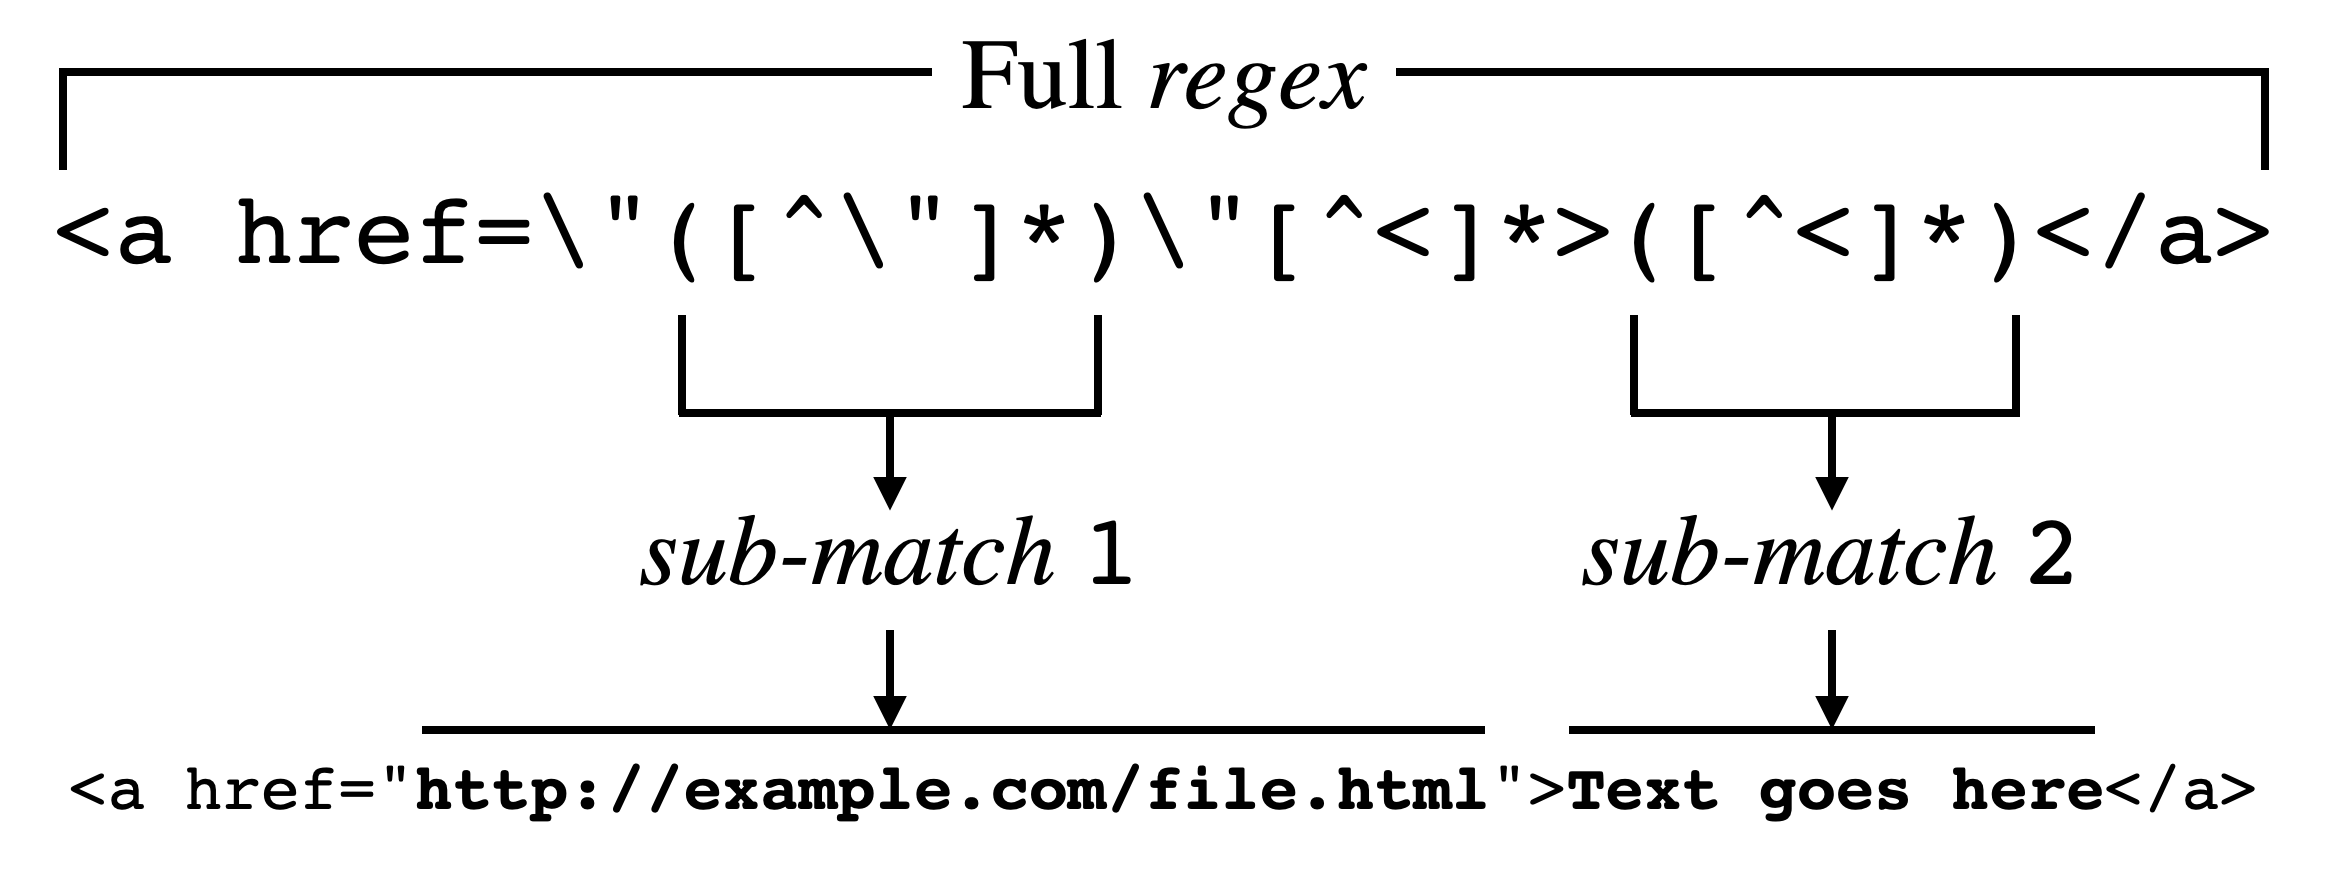
\includegraphics[width=0.8\textwidth]{content/chapter7/images/1.png}\\
Figure 7.1 – A Regular Expression with sub-matches
\end{center}

This allows us to match a string and use parts of that string as our results:

\begin{lstlisting}[style=styleCXX]
sregex_token_iterator it{ in.begin(), in.end(), link_re, {1, 2}
};
\end{lstlisting}

The sub-matches are numbered, beginning with 1. Sub-match 0 is a special value that represents the entire match.

Once we have our iterator, we use it as we would any other iterator:

\begin{lstlisting}[style=styleCXX]
for(It end_it{}; it != end_it; ) {
	const string link{ *it++ };
	if(it == end_it) break;
	const string desc{ *it++ };
	cout << format("{:.<24} {}\n", desc, link);
}
\end{lstlisting}

This simply steps through our results via the regex iterator, giving us the formatted output:

\begin{tcblisting}{commandshell={}}
Bill Weinman............ https://bw.org/
courses................. https://bw.org/courses/
music................... https://bw.org/music/
books................... https://packt.com/
back to the internet.... https://duckduckgo.com/
\end{tcblisting}












